\clearpage
\section{Mockups}\label{sec:interfaccia}
Le schermate seguenti sono state acquisite dall'applicazione JavaFX corrente, avviata con il database dimostrativo in memoria. I dati visualizzati appartengono al popolamento di prova. Le viste sono presentate nell'ordine in cui l'utente le incontra e poi raggruppate per ruolo, come nella relazione ChargeNet.

\newcommand{\uiscreen}[3]{%
  \begin{figure}[H]
    \centering
    \includegraphics[width=\textwidth,height=.64\textheight,keepaspectratio]{mockups/#1}
    \caption{#2}\label{#3}
  \end{figure}}
\newcommand{\uiauthscreen}[4]{%
  \begin{figure}[H]
    \centering
    \includegraphics[trim=#4,clip,width=.80\textwidth,height=.64\textheight,keepaspectratio]{mockups/#1}
    \caption{#2}\label{#3}
  \end{figure}}

\subsection{Autenticazione}

\filbreak
\subsubsection{Schermata iniziale}
La pagina di benvenuto è il punto di ingresso dell'applicazione e offre i collegamenti all'accesso e alla creazione di un account.
\uiauthscreen{00-benvenuto.png}{Schermata iniziale di DriveHub.}{fig:ui-benvenuto}{340bp 180bp 340bp 180bp}

\filbreak
\subsubsection{Accesso}
La schermata di login richiede email e password. Dopo la verifica delle credenziali, l'utente viene indirizzato all'area corrispondente al proprio ruolo.
\uiauthscreen{01-accesso.png}{Schermata di accesso.}{fig:ui-accesso}{410bp 20bp 410bp 20bp}

\filbreak
\subsubsection{Registrazione}
La registrazione raccoglie nome, cognome, email, password e ruolo. Per il Customer viene creato automaticamente un conto dimostrativo. La scelta pubblica dei ruoli Salesman e Manager è una semplificazione del prototipo.
\uiauthscreen{02-registrazione.png}{Schermata di registrazione.}{fig:ui-registrazione}{410bp 20bp 410bp 20bp}

\subsection{Area Customer}

\filbreak
\subsubsection{Catalogo veicoli}
Il catalogo presenta i veicoli con targa, VIN, modello, anno, chilometri, prezzo e stato. Il Customer può cercare per testo, filtrare per modalità e scegliere un veicolo per avviare acquisto, noleggio o test drive.
\uiscreen{customer-catalogo.png}{Catalogo dei veicoli nell'area Customer.}{fig:ui-catalogo}

\filbreak
\subsubsection{Acquisti e richieste}
La scheda distingue le richieste ancora aperte dallo storico delle compravendite. Per una richiesta di acquisto autorizzata il Customer può pagare il saldo; può anche annullare l'acquisto con rimborso parziale dell'acconto.
\uiscreen{customer-acquisti.png}{Richieste di acquisto e storico del Customer.}{fig:ui-acquisti}

\filbreak
\subsubsection{Noleggi e test drive}
Le due operazioni condividono una scheda: il noleggio richiede un intervallo di date, mentre il test drive richiede una data e uno slot di un'ora fra le 09:00 e le 16:00. Le tabelle sottostanti mostrano le prenotazioni del Customer.
\uiscreen{customer-noleggi-test-drive.png}{Prenotazione di noleggi e test drive.}{fig:ui-noleggi-test-drive}

\filbreak
\subsubsection{Proposta di vendita del proprio veicolo}
Il Customer seleziona marca e modello e inserisce VIN, targa, chilometri e anno. Il sistema calcola una valutazione prima dell'invio della proposta, che sarà esaminata dal Salesman.
\uiscreen{customer-cessione.png}{Modulo di proposta di un veicolo alla concessionaria.}{fig:ui-cessione}

\filbreak
\subsubsection{Conto dimostrativo}
La scheda mostra IBAN e saldo del conto usato per gli addebiti e gli accrediti delle operazioni. I comandi di deposito e prelievo modificano soltanto il conto interno al prototipo.
\uiscreen{customer-conto.png}{Conto dimostrativo del Customer.}{fig:ui-conto}

\filbreak
\subsubsection{Profilo}
Il Customer può aggiornare email e password o eliminare il proprio account, confermando le modifiche con la password corrente.
\uiscreen{customer-profilo.png}{Gestione del profilo Customer.}{fig:ui-customer-profilo}

\clearpage
\subsection{Area Salesman}

\filbreak
\subsubsection{Veicoli in attesa}
La prima scheda raccoglie i veicoli proposti dai clienti e in stato \code{WAITING}. Il Salesman può approvare la proposta, liquidando il cliente e mettendo il veicolo in vendita, oppure rifiutarla.
\uiscreen{salesman-proposte.png}{Coda delle proposte nell'area Salesman.}{fig:ui-salesman-proposte}

\filbreak
\subsubsection{Richieste di acquisto}
Il Salesman consulta gli acconti versati e autorizza le richieste d'acquisto. L'autorizzazione assegna il venditore e fissa la scadenza del saldo a un mese.
\uiscreen{salesman-richieste.png}{Richieste di acquisto e autorizzazione del saldo.}{fig:ui-salesman-richieste}

\filbreak
\subsubsection{Stato dei veicoli}
Questa scheda consente di cambiare la modalità di un veicolo fra vendita e noleggio. Il passaggio da noleggio a vendita comporta l'annullamento dei noleggi futuri e il relativo rimborso.
\uiscreen{salesman-stato-veicoli.png}{Gestione dello stato dei veicoli.}{fig:ui-salesman-stato}

\filbreak
\subsubsection{Panoramica prenotazioni}
Il Salesman vede le prenotazioni di noleggio e di test drive. La schermata fornisce una vista operativa delle richieste registrate, senza introdurre ulteriori stati di lavorazione.
\uiscreen{salesman-panoramica.png}{Panoramica di noleggi e test drive.}{fig:ui-salesman-panoramica}

\filbreak
\subsubsection{Profilo}
Anche il Salesman dispone dei comandi per cambiare email e password e per eliminare l'account.
\uiscreen{salesman-profilo.png}{Gestione del profilo Salesman.}{fig:ui-salesman-profilo}

\clearpage
\subsection{Area Manager}

\filbreak
\subsubsection{Parco veicoli}
Il Manager consulta tutti i veicoli e può applicare o rimuovere uno sconto sul singolo esemplare. Nella stessa scheda può aggiungere un nuovo veicolo al catalogo o eliminare quello selezionato.
\uiscreen{manager-parco-veicoli.png}{Parco veicoli e sconti individuali.}{fig:ui-manager-parco}

\filbreak
\subsubsection{Marche e modelli}
La schermata permette di mantenere l'anagrafica delle marche e dei modelli e di impostare sconti a livello di modello, distinti da quelli del singolo veicolo.
\uiscreen{manager-marche-modelli.png}{Gestione di marche, modelli e sconti.}{fig:ui-manager-modelli}

\filbreak
\subsubsection{Registro delle operazioni}
Il registro raccoglie vendite concluse, acquisizioni di veicoli dai clienti e penali per acquisti annullati o scaduti. Importo e tipo di operazione sono mostrati nella stessa tabella.
\uiscreen{manager-vendite.png}{Registro delle vendite e delle altre operazioni economiche.}{fig:ui-manager-vendite}

\filbreak
\subsubsection{Profilo}
Il Manager può modificare le proprie credenziali e gestire l'account dalla scheda dedicata.
\uiscreen{manager-profilo.png}{Gestione del profilo Manager.}{fig:ui-manager-profilo}

\clearpage
\section{Page Navigation Diagram}
Il diagramma mostra i percorsi tra la pagina iniziale, l'accesso, la registrazione e le aree dei tre ruoli. Dopo l'autenticazione, il sistema apre l'area corrispondente al ruolo dell'utente. I riquadri sotto Customer, Salesman e Manager rappresentano le schede interne alle rispettive aree; il logout riporta alla pagina iniziale.
\begin{figure}[H]
  \centering
  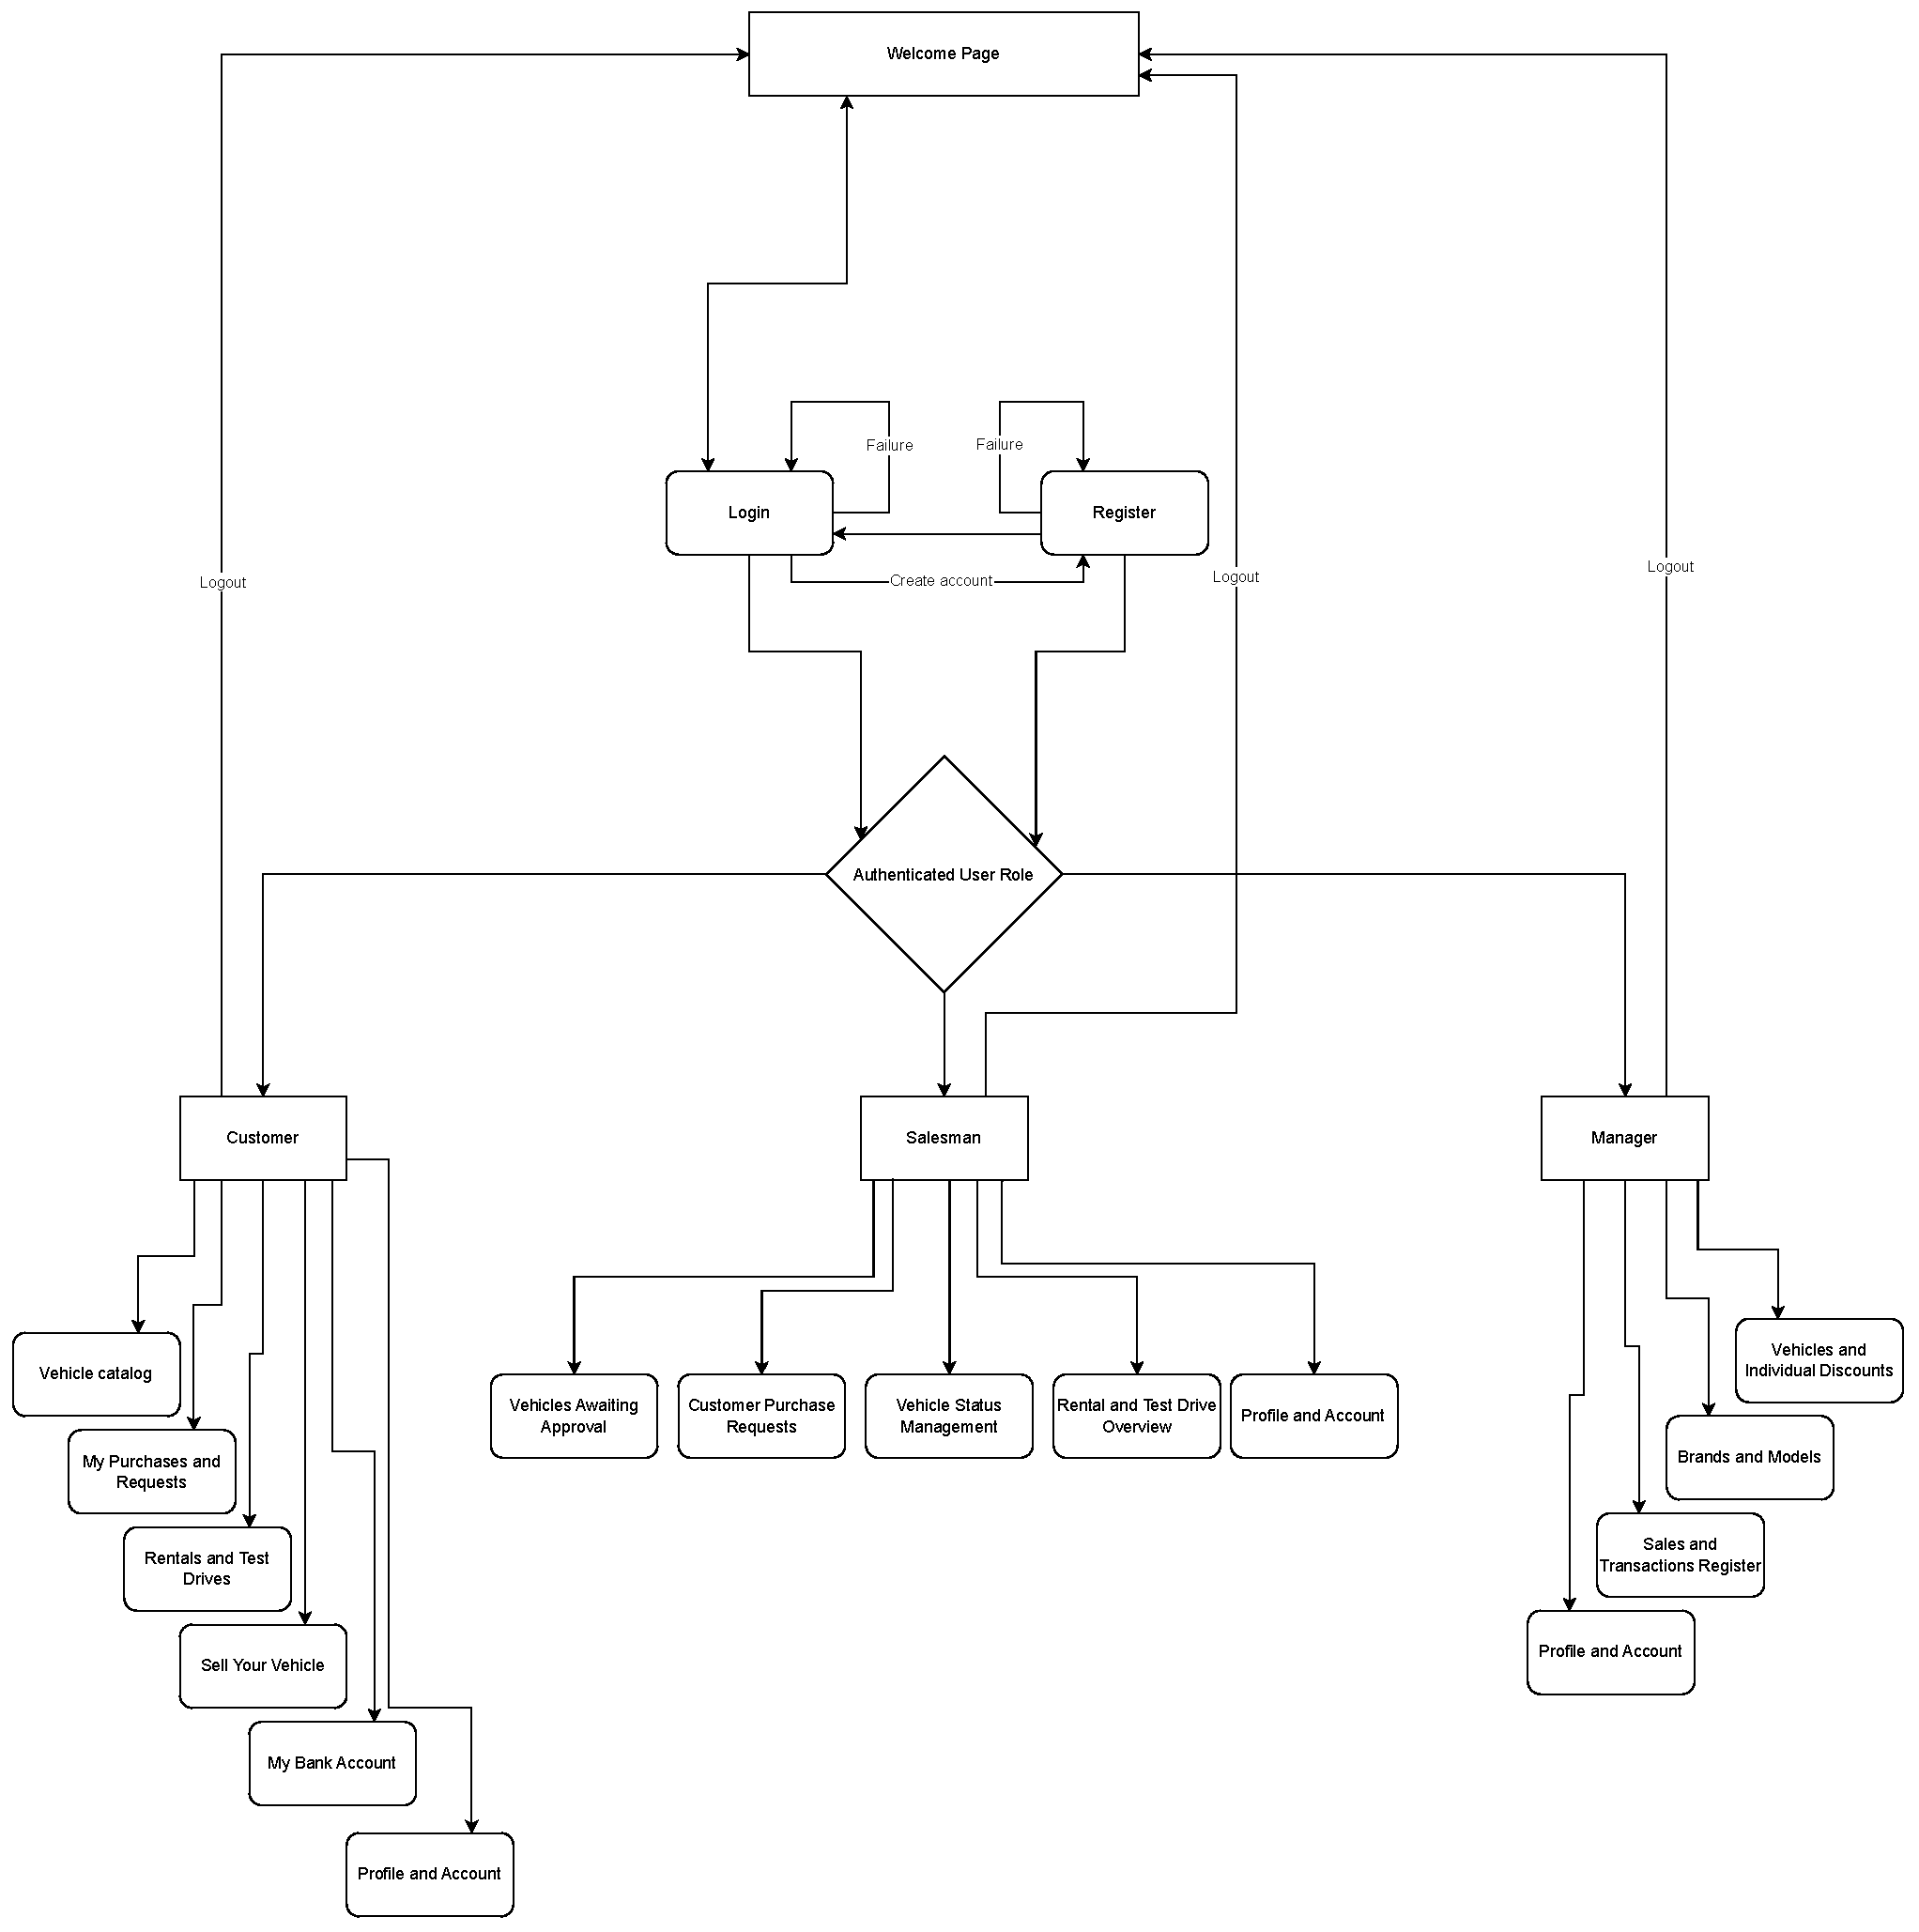
\includegraphics[width=\textwidth,height=.74\textheight,keepaspectratio]{page-navigation-original.pdf}
  \caption{Diagramma di navigazione delle pagine e delle schede di DriveHub.}\label{fig:navigazione-corrente}
\end{figure}
